\subsection{SymPy Gamma}\label{sympy-gamma}

SymPy Gamma is a simple web application that runs on Google App Engine 
that executes and displays the results of SymPy expressions as well as
additional related computations, in a fashion similar to that of
Wolfram\textbar{}Alpha. For instance, entering an integer will display
prime factors, digits in the base-10 expansion, and a factorization
diagram. Entering a function will give its docstring; in general,
entering an arbitrary expression will provide the derivative, integral,
series expansion, plot, and roots.

SymPy Gamma also has several additional features than just computing the
results using SymPy.

\begin{itemize}
\item
  It displays integration steps, differentiation steps in detail, which
  can be viewed below:\par
\begin{minipage}{\textwidth}
    \centering
    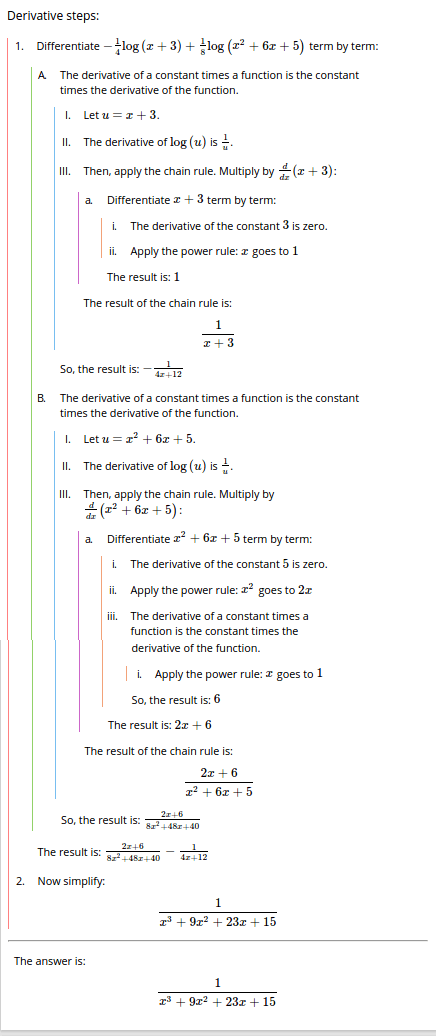
\includegraphics[width=0.7\textwidth]{derivative_steps.png}
    \captionof{figure}{Derivative steps of $\frac{\mathrm{d}}{\mathrm{d} x}\left (\frac{-\log(x + 3)}{4} + \frac{\log(x^2 + 6x + 5)}{8}\right)$}
\end{minipage}
\item
  It also displays the factor tree diagrams for numbers, which is also
  illustrated through this image:\par
\begin{minipage}{\textwidth}
    \centering
    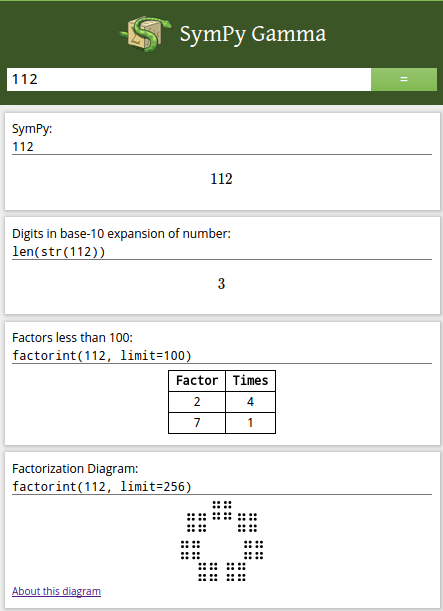
\includegraphics[width=0.7\textwidth]{factor_tree_diagram.png}
    \captionof{figure}{Factor Tree Diagram of \textbf{112}}
\end{minipage}
\item
  SymPy Gamma also saves user search queries, and offers many such 
  similar features for free, which Wolfram\textbar{}Alpha only offers 
  to its paid users.
\end{itemize}
Every input query from the user on SymPy Gamma is first, parsed by its
own parser, which handles several different forms of function names,
which SymPy as a library doesn't support. For instance, SymPy Gamma
supports queries like - \texttt{sin\ x}, whereas SymPy doesn't support
this, and supports only \texttt{sin(x)}.

This parser, then converts the input query to the resultant SymPy
readable code, which is then eventually processed by SymPy and the
result is finally formatted in LaTeX and displayed on the SymPy Gamma
web-app.